%!TEX root = ../Thesis.tex
\chapter{Bilinear Model}
\section{Bilinear System}
\label{sec:bilinear_system}

In the bilinear formulation considered in this work, the system matrices depend on a time-varying variable \(v_k\). The discrete-time state-space model is written as

\begin{align}
    x_{k+1} &= A(v_k)x_k + B(v_k)u_k \label{eq:bilinear_state}\\
    y_k &= Cx_k \label{eq:bilinear_output}
\end{align}

For compactness, the time-varying system matrices are denoted by

\begin{equation}
    A_k = A(v_k),
    \qquad
    B_k = B(v_k)
\end{equation}

The state equation can therefore be written as

\begin{equation}
    x_{k+1} = A_k x_k + B_k u_k
    \label{eq:bilinear_compact}
\end{equation}

Unlike the LTI case, where \(A\) and \(B\) remain constant over the prediction horizon, the matrices \(A_k\) and \(B_k\) may change at every prediction step according to the corresponding value of \(v_k\).

\subsection{State and Output Prediction}

Starting from the initial state \(x_0\), the first predicted state is

\begin{equation}
    x_1 = A_0x_0 + B_0u_0
\end{equation}

The corresponding output is

\begin{equation}
    y_1
    =
    Cx_1
    =
    CA_0x_0 + CB_0u_0
    \label{eq:bilinear_y1}
\end{equation}

At the second prediction step,

\begin{align}
    x_2
    &= A_1x_1+B_1u_1 \\
    &= A_1(A_0x_0+B_0u_0)+B_1u_1 \\
    &= A_1A_0x_0+A_1B_0u_0+B_1u_1
\end{align}

Therefore,

\begin{align}
    y_2
    &= Cx_2 \\
    &= CA_1A_0x_0
    +CA_1B_0u_0
    +CB_1u_1
    \label{eq:bilinear_y2}
\end{align}

Similarly, the third predicted state is

\begin{align}
    x_3
    &=
    A_2x_2+B_2u_2 \\
    &=
    A_2A_1A_0x_0
    +A_2A_1B_0u_0
    +A_2B_1u_1
    +B_2u_2
\end{align}

and hence

\begin{align}
    y_3
    &=
    CA_2A_1A_0x_0
    +CA_2A_1B_0u_0 \nonumber\\
    &\quad
    +CA_2B_1u_1
    +CB_2u_2
\end{align}

Following the same recursive structure, the state at prediction step \(k\) can be expressed as

\begin{equation}
    x_k
    =
    \left(
        \prod_{j=0}^{k-1} A_j
    \right)x_0
    +
    \sum_{i=0}^{k-1}
    \left(
        \prod_{j=i+1}^{k-1} A_j
    \right)
    B_i u_i
    \label{eq:bilinear_xk}
\end{equation}

where the matrix products are ordered such that

\begin{equation}
    \prod_{j=0}^{k-1}A_j
    =
    A_{k-1}A_{k-2}\cdots A_0
\end{equation}

For \(i=k-1\), the product multiplying \(B_{k-1}u_{k-1}\) is interpreted as the identity matrix.

Using \(y_k=Cx_k\), the corresponding predicted output becomes

\begin{equation}
    y_k
    =
    C
    \left(
        \prod_{j=0}^{k-1} A_j
    \right)x_0
    +
    \sum_{i=0}^{k-1}
    C
    \left(
        \prod_{j=i+1}^{k-1} A_j
    \right)
    B_i u_i
    \label{eq:bilinear_yk}
\end{equation}

\subsection{Stacked Prediction Formulation}

As in the LTI case, the future outputs and control inputs over a prediction horizon \(N\) are collected into stacked vectors:

\begin{equation}
    Y =
    \begin{bmatrix}
        y_1 \\
        y_2 \\
        \vdots \\
        y_N
    \end{bmatrix},
    \qquad
    U =
    \begin{bmatrix}
        u_0 \\
        u_1 \\
        \vdots \\
        u_{N-1}
    \end{bmatrix}
\end{equation}

Using the previously derived output equations, the stacked prediction can be written as

\begin{equation}
    Y
    =
    \Phi(V)x_0
    +
    \Gamma(V)U,
    \label{eq:bilinear_stacked}
\end{equation}

where

\begin{equation}
    V =
    \begin{bmatrix}
        v_0 &
        v_1 &
        \cdots &
        v_{N-1}
    \end{bmatrix}^{T}
\end{equation}

contains the values determining the system matrices over the prediction horizon.

The state-dependent prediction matrix is

\begin{equation}
    \Phi(V)
    =
    \begin{bmatrix}
        CA_0 \\
        CA_1A_0 \\
        CA_2A_1A_0 \\
        \vdots \\
        CA_{N-1}A_{N-2}\cdots A_0
    \end{bmatrix}
    \label{eq:bilinear_phi}
\end{equation}

The input prediction matrix is

\begin{equation}
\resizebox{0.9\linewidth}{!}{$ % Denklemi satır genişliğinin %90'ına sığdırır
\Gamma(V)
=
\begin{bmatrix}
CB_0 & 0 & 0 & \cdots & 0 \\[2mm]
CA_1B_0 & CB_1 & 0 & \cdots & 0 \\[2mm]
CA_2A_1B_0 & CA_2B_1 & CB_2 & \cdots & 0 \\
\vdots & \vdots & \vdots & \ddots & \vdots \\[2mm]
CA_{N-1}\cdots A_1B_0 & CA_{N-1}\cdots A_2B_1 & CA_{N-1}\cdots A_3B_2 & \cdots & CB_{N-1}
\end{bmatrix}
$}
\label{eq:bilinear_gamma}
\end{equation}
Consequently, the compact prediction equation is

\begin{equation}
    \boxed{
        Y = \Phi(V)x_0+\Gamma(V)U
    }
    \label{eq:bilinear_prediction}
\end{equation}

\section{Optimal Control Problem}
\label{sec:bilinear_optimal_control}

For the bilinear system, both the control sequence \(U\) and the scheduling-variable sequence \(V\) are treated as optimization variables. The decision vector is therefore defined as

\begin{equation}
    z =
    \begin{bmatrix}
        U \\
        V
    \end{bmatrix}
\end{equation}

Using the bilinear stacked prediction model,

\begin{equation}
    Y_{\mathrm{pred}}
    =
    \Phi(V)x_0
    +
    \Gamma(V)U
\end{equation}

the tracking error is defined as

\begin{equation}
    e
    =
    Y_{\mathrm{pred}}
    -
    \bar{Y}
\end{equation}

The quadratic objective function is then written as

\begin{equation}
    \phi(z)
    =
    e^TQe
    +
    U^TR_UU
    +
    V^TR_VV,
    \label{eq:bilinear_cost_compact}
\end{equation}

where \(Q \succeq 0\) penalizes the output tracking error, while
\(R_U \succ 0\) and \(R_V \succ 0\) penalize the magnitudes of the control and scheduling-variable sequences, respectively.

Substituting the prediction model into the cost function gives

\begin{align}
    \phi(U,V)
    &=
    \left(
        \Phi(V)x_0
        +
        \Gamma(V)U
        -
        \bar{Y}
    \right)^T
    Q
    \left(
        \Phi(V)x_0
        +
        \Gamma(V)U
        -
        \bar{Y}
    \right)
    \nonumber\\
    &\quad
    +
    U^TR_UU
    +
    V^TR_VV
    \label{eq:bilinear_cost_expanded}
\end{align}

The optimal control and scheduling sequences are therefore obtained from

\begin{equation}
    \boxed{
    (U^\ast,V^\ast)
    =
    \arg\min_{U,V}
    \phi(U,V)
    }
    \label{eq:bilinear_optimization}
\end{equation}

In the LTI case, the prediction matrices \(\Phi\) and \(\Gamma\) are constant. As a result, the cost function is quadratic in \(U\), and the optimal solution can be obtained analytically by setting the gradient equal to zero.

For the bilinear system, however, both \(\Phi(V)\) and \(\Gamma(V)\) depend on the optimization variable \(V\). Consequently, the predicted output depends nonlinearly on the joint decision vector \(z=[U^T \; V^T]^T\). The resulting optimization problem is therefore generally nonlinear and does not admit the same closed-form solution used for the LTI system.

\subsection{Numerical Solution Using SLSQP}

The nonlinear optimization problem in \cref{eq:bilinear_optimization} is solved numerically using Sequential Least Squares Programming (SLSQP).

SLSQP is a gradient-based constrained optimization method that solves a sequence of local quadratic approximations of the original nonlinear problem. At each iteration, the algorithm updates the decision variables while attempting to reduce the objective function and satisfy the imposed constraints.

The optimization variable is

\begin{equation}
    z =
    \begin{bmatrix}
        U \\
        V
    \end{bmatrix}
\end{equation}

with an initial guess

\begin{equation}
    z^{(0)}
    =
    \begin{bmatrix}
        U^{(0)} \\
        V^{(0)}
    \end{bmatrix}
\end{equation}

At each SLSQP iteration, the current sequence \(V\) is used to construct the time-varying matrices

\begin{equation}
    A_k=A(v_k),
    \qquad
    B_k=B(v_k)
\end{equation}

and consequently the prediction matrices

\begin{equation}
    \Phi(V),
    \qquad
    \Gamma(V)
\end{equation}

The predicted output is then evaluated as

\begin{equation}
    Y_{\mathrm{pred}}
    =
    \Phi(V)x_0
    +
    \Gamma(V)U
\end{equation}

and the objective function \(\phi(U,V)\) is computed.

The optimizer repeatedly updates \(U\) and \(V\) until a convergence criterion is satisfied, resulting in the numerical solution

\begin{equation}
    z^\ast
    =
    \begin{bmatrix}
        U^\ast \\
        V^\ast
    \end{bmatrix}
\end{equation}

\section{Open-Loop Implementation}
\label{sec:bilinear_open_loop}

The open-loop implementation of the bilinear controller follows the same general structure as the open-loop implementation introduced for the LTI system. However, the optimal control problem is solved numerically for both \(U\) and \(V\), rather than analytically for \(U\) alone.

The implementation procedure can therefore be summarized as follows:

\begin{enumerate}
    \item Select the prediction horizon \(N\), reference trajectory \(\bar{Y}\), weighting matrices \(Q\), \(R_U\), \(R_V\), and the initial state \(x_0\).
    \item Define the bounds and initial guesses for the optimization variables \(U\) and \(V\).
    \item For a candidate sequence \(V\), construct the time-varying matrices
    \[
        A_k=A(v_k),
        \qquad
        B_k=B(v_k)
    \]
    \item Construct the prediction matrices \(\Phi(V)\) and \(\Gamma(V)\).
    \item Construct the nonlinear objective function \(\phi(U,V)\).
    \item Solve the optimization problem numerically using SLSQP to obtain \(U^\ast\) and \(V^\ast\).
    \item Apply the components of \(U^\ast\) and \(V^\ast\) sequentially to the bilinear system.
    \item Compare the resulting output trajectory with the reference trajectory.
\end{enumerate}

At each simulation step, the optimized values are applied according to

\begin{align}
    x_{k+1}
    &=
    A(v_k^\ast)x_k
    +
    B(v_k^\ast)u_k^\ast \\
    y_k
    &=
    Cx_k
\end{align}

Since the controller operates in open loop, the optimization is not updated after the simulation begins. Therefore, the sequences \(U^\ast\) and \(V^\ast\) are determined entirely from the initial state and the prescribed reference trajectory.

\subsection{Results}
\label{subsec:bilinear_open_loop_results}

The bilinear open-loop controller was evaluated using the system

\begin{equation}
    x_{k+1}
    =
    A(v_k)x_k
    +
    B(v_k)u_k,
    \qquad
    y_k=Cx_k
\end{equation}

with

\begin{equation}
    A(v)
    =
    \begin{bmatrix}
        0.9 & v \\
        0.0 & 0.5
    \end{bmatrix}
\end{equation}

\begin{equation}
    B(v)
    =
    \begin{bmatrix}
        0 \\
        1
    \end{bmatrix},
    \qquad
    C=
    \begin{bmatrix}
        1.0 & 0.0
    \end{bmatrix}
\end{equation}

The initial state was selected as

\begin{equation}
    x_0
    =
    \begin{bmatrix}
        1.0 \\
        0.0
    \end{bmatrix}
\end{equation}

The optimization bounds were chosen as

\begin{align}
    -5.0 &\leq u_k \leq 5.0 \\
    -10.0 &\leq v_k \leq 10.0
\end{align}

The control penalties were selected as

\begin{equation}
    R_U = 0.1,
    \qquad
    R_V = 0.1
\end{equation}


\begin{figure}[H]
    \centering
    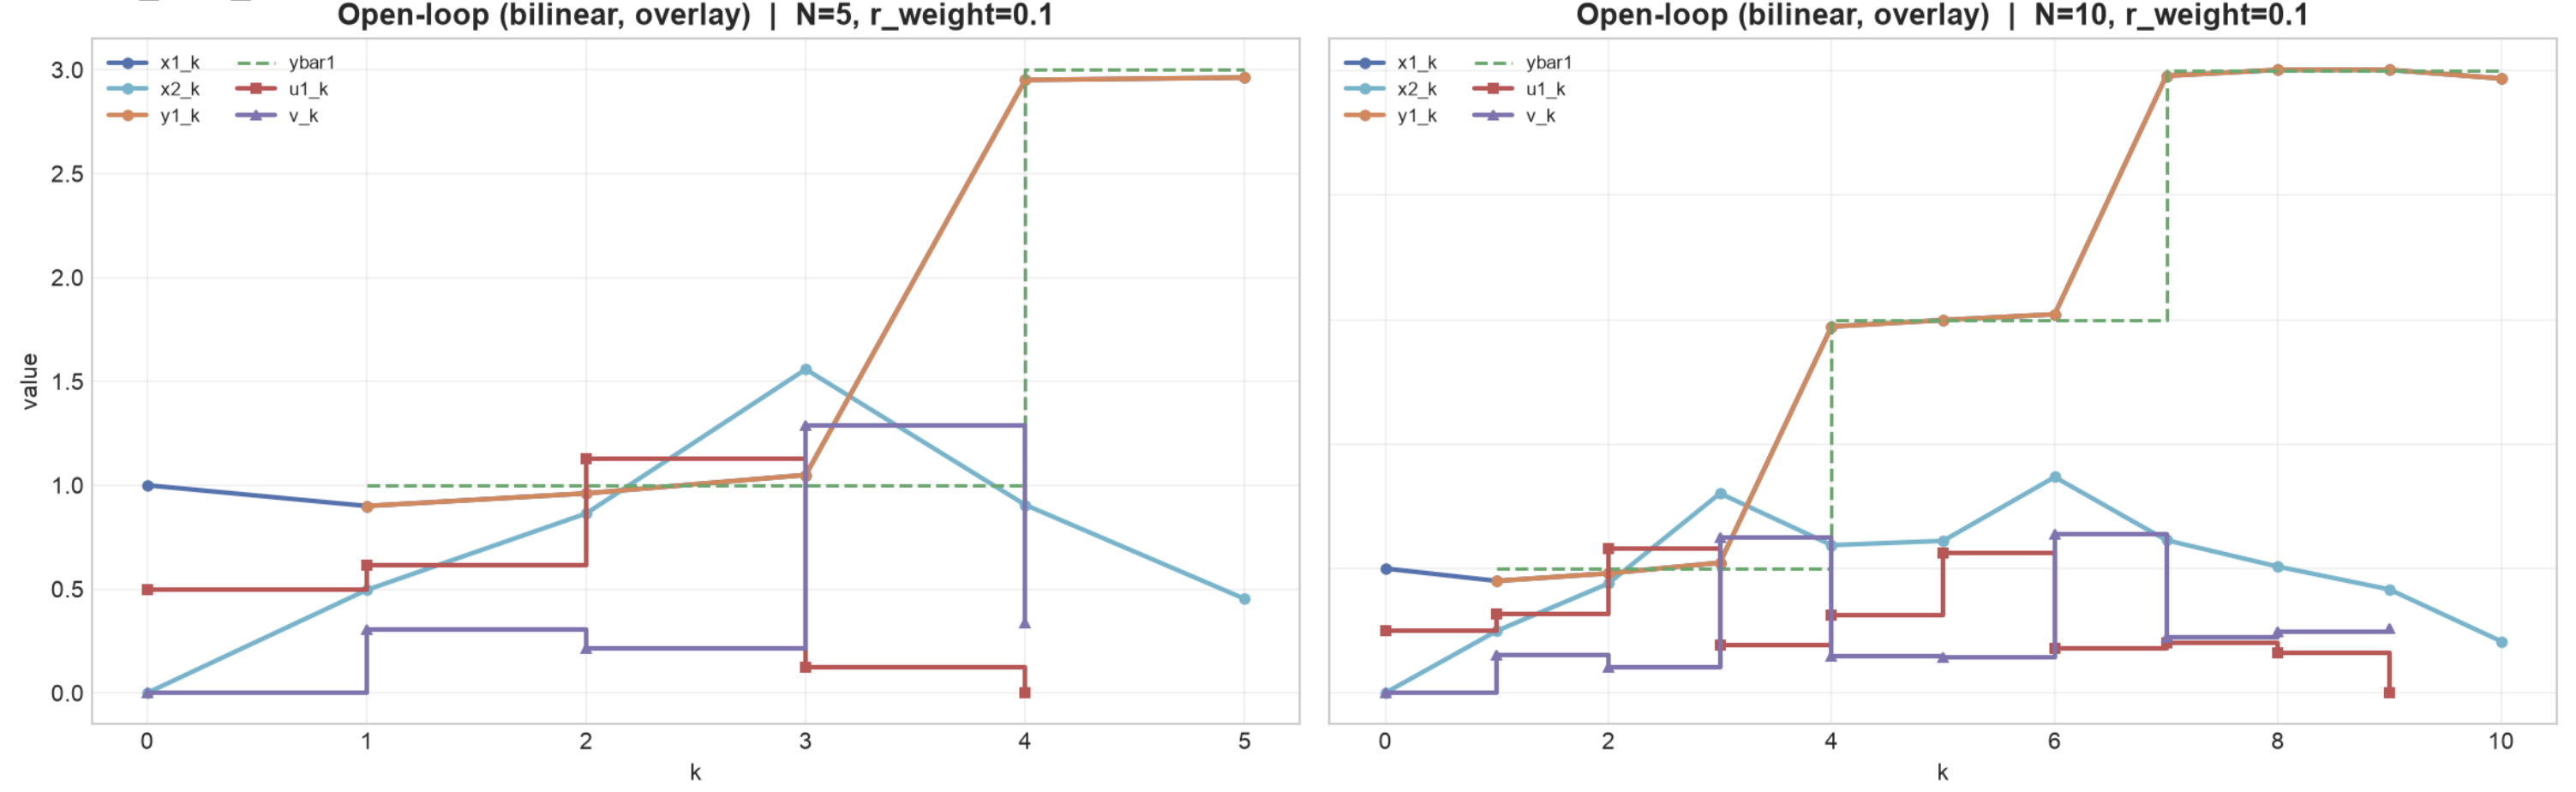
\includegraphics[width=1.0\textwidth]{graphics/Bilinear_Open_Loop.png}
    \caption{Open-loop output tracking performance of the bilinear system, left-side is the case when N=5, and right-side is the case when N=10}
    \label{fig:bilinear_open_loop_output}
\end{figure}


\section{Closed-Loop Implementation}
\label{sec:bilinear_closed_loop}

The closed-loop implementation of the bilinear controller follows the same receding-horizon principle introduced for the LTI system. However, in the bilinear case, both the control sequence \(U\) and the scheduling-variable sequence \(V\) are optimized at every sampling instant.

At time step \(k\), the current state \(x_k\) is used together with the reference trajectory over the prediction horizon. The nonlinear optimization problem is then solved numerically using SLSQP. Only the first elements of the optimal sequences are applied to the system. At the next time step, the state is updated and the complete optimization problem is solved again.



Only the first control values are applied to the system. Using the selection matrix \(\Pi\),

\begin{align}
    u_k &= \Pi U_c^\ast \\
    v_k &= \Pi V_c^\ast
\end{align}



After the state is updated, the prediction horizon is shifted forward by one step and the optimization problem is solved again using the new state \(x_{k+1}\).

The closed-loop bilinear control procedure can therefore be summarized as follows:

\begin{enumerate}
    \item Select \(N\), \(N_c\), \(N_{\mathrm{end}}\), \(Q\), \(R_U\), \(R_V\), the reference trajectory, and \(x_0\).

    \item Define the bounds and initial guesses for the optimization variables \(U_c\) and \(V_c\), and construct the control-horizon mapping matrix \(T\).

    \item At time step \(k\), construct the reference vector \(\bar{Y}_k\) over the current prediction horizon.

    \item For the current candidate sequence \(V_c\), construct
    \(
        V_{\mathrm{full}} = TV_c
    \)
    and the corresponding time-varying system matrices
    \(
        A_i=A(v_i),
        \quad
        B_i=B(v_i).
    \)

    \item Construct the prediction matrices
    \(
        \Phi(V_{\mathrm{full}})
        \quad \text{and} \quad
        \Gamma(V_{\mathrm{full}}).
    \)

    \item Solve the nonlinear optimization problem using SLSQP to obtain
    \(
        U_c^\ast
        \quad \text{and} \quad
        V_c^\ast.
    \)

    \item Apply only the first elements of the optimal sequences:
    \(
        u_k = \Pi U_c^\ast,
        \quad
        v_k = \Pi V_c^\ast.
    \)

    \item Update the system state and output:
    \(
        x_{k+1}
        =
        A(v_k)x_k
        +
        B(v_k)u_k,
        \quad
        y_k=Cx_k.
    \)

    \item Shift the prediction horizon and repeat the optimization for \(k+1\) until \(k=N_{\mathrm{end}}-1\).
\end{enumerate}

\subsection{Results}
\label{subsec:bilinear_closed_loop_results}

The closed-loop bilinear controller was evaluated using the same system and parameter settings as in the open-loop implementation.


However, the sequences \(U^\ast\) and \(V^\ast\) are not computed only once. Instead, a new nonlinear optimization problem is solved at every sampling instant using the current state of the system.

\begin{figure}[H]
    \centering
    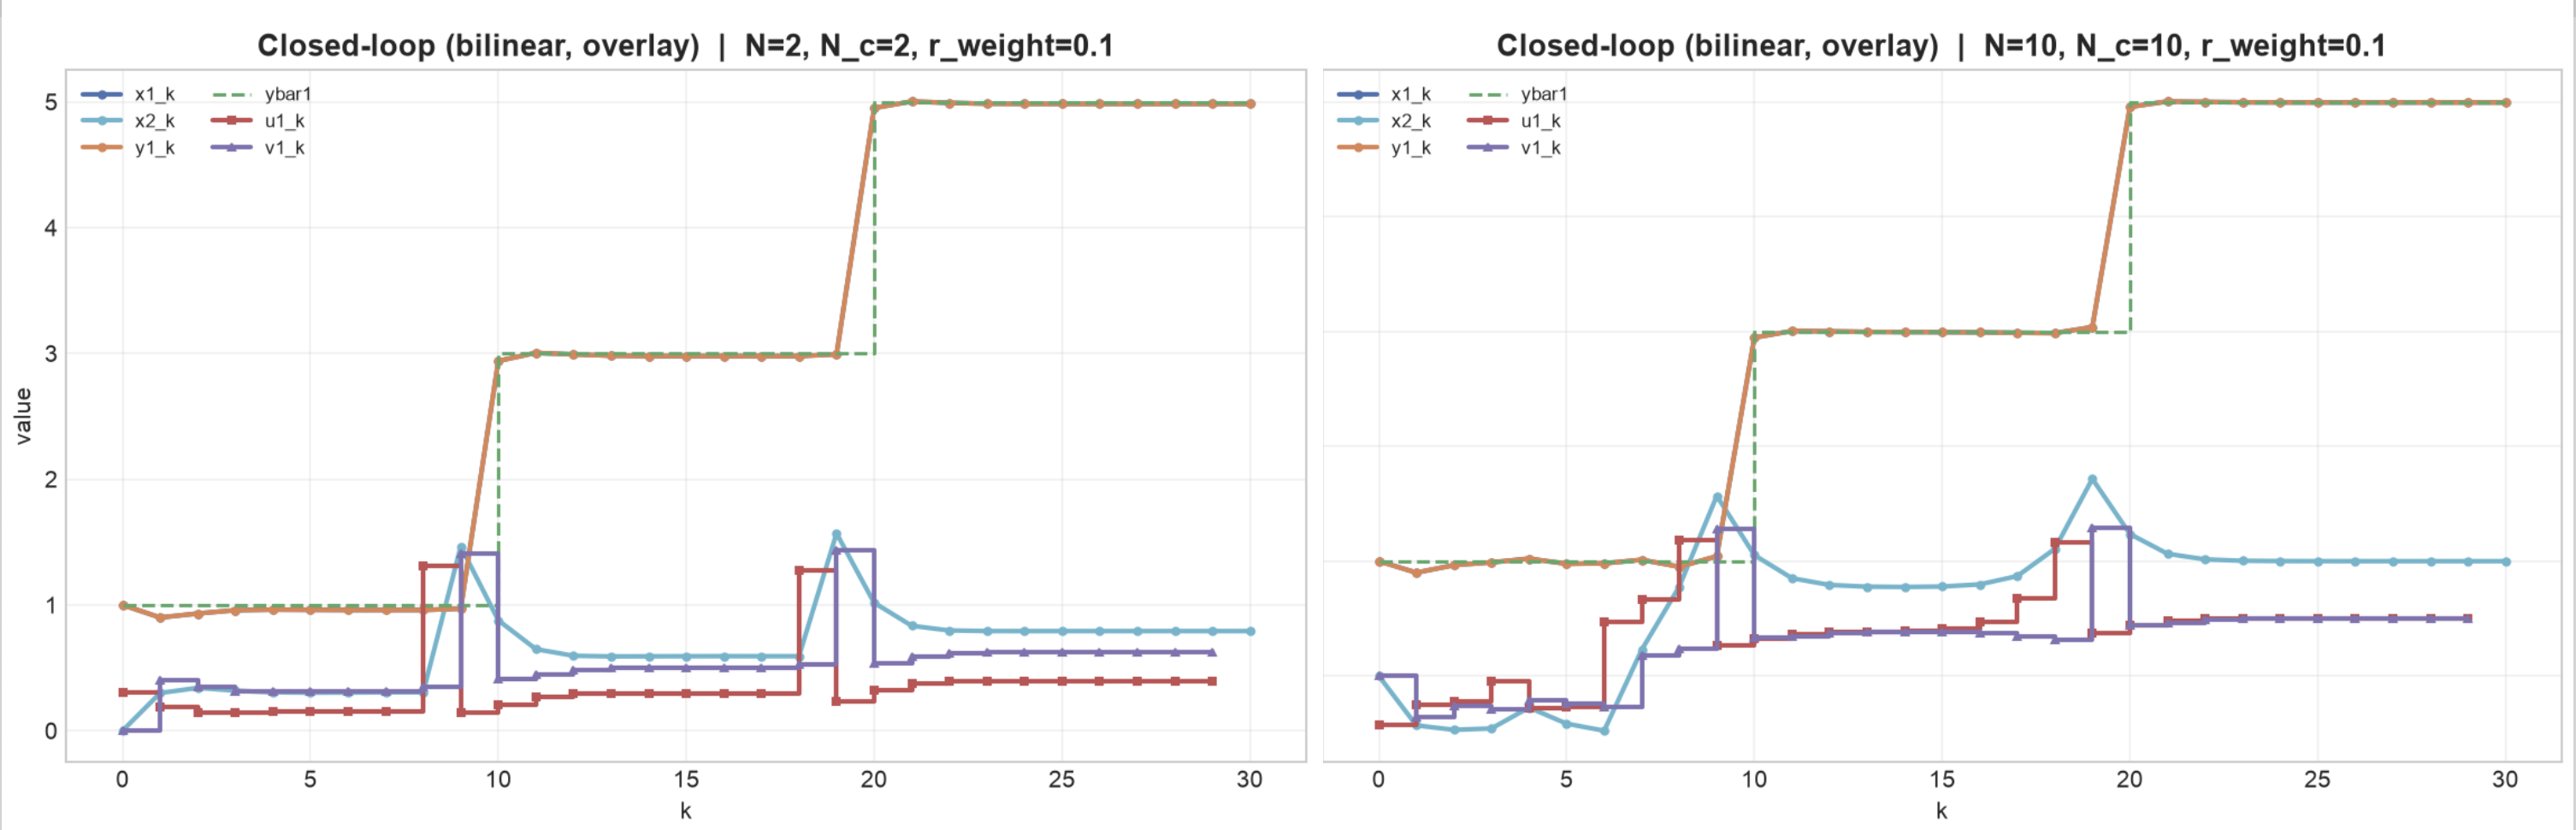
\includegraphics[width=1.0 \textwidth]{graphics/Bilinear_Closed_Loop.png}
    \caption{Closed-loop output tracking performance of the bilinear system, left-side is the case when N=2, and right-side is the case when N=10}
    \label{fig:bilinear_closed_loop_output}
\end{figure}

